\documentclass[border=3pt]{standalone}
\usepackage{tikz}
\usetikzlibrary{decorations.pathreplacing,patterns, arrows}
\definecolor{greengreen}{rgb}{0.0, 0.42, 0.24}
%%%%%%%%%%%%%%%%%%%%%%%%%%%%%%%%%%%%%%%%%%%%%%%%%%%%%%%%%%%%%%%%%
\begin{document}
%%%%%%%%%%%%%%%%%%%%%%%%%%%%%%%%%%%%%%%%%%%%%%%%%%%%%%%%%%%%%%%%%
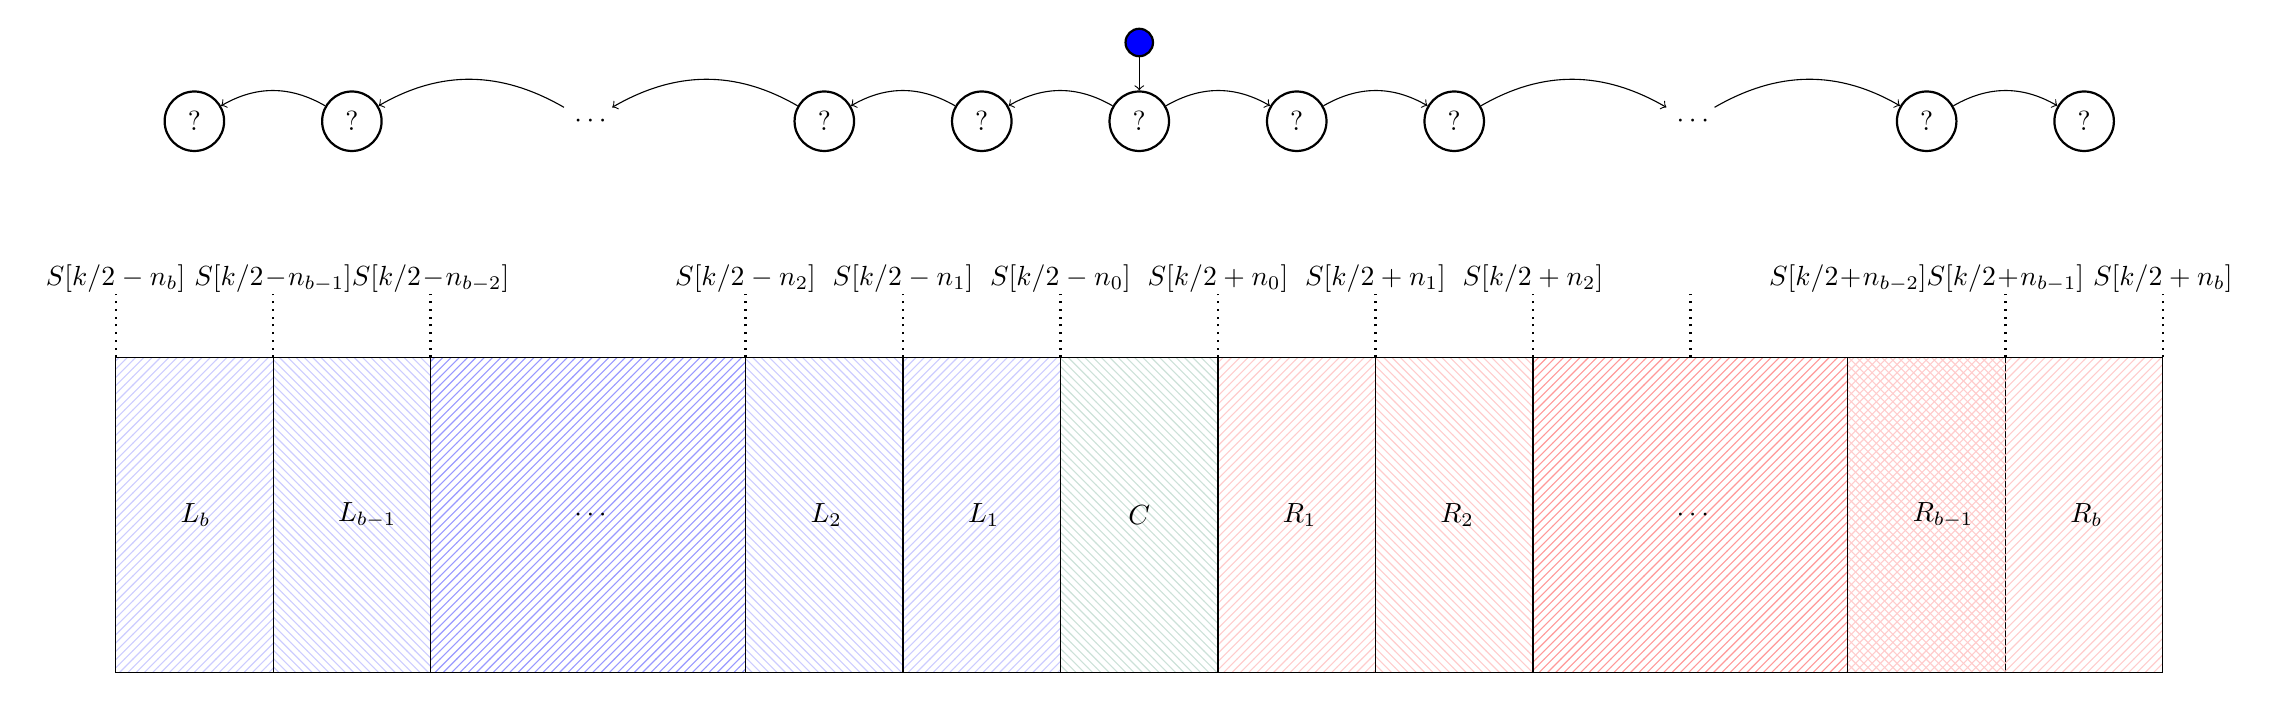
\begin{tikzpicture}[every node/.style={align=center, thick},
red/.style={fill=red,draw,circle,inner sep=0pt},
blue/.style={fill=blue,draw,circle,inner sep=0pt},
 text width = .35cm]
%================================================================
%	Boxes
% \draw[very thick] (0,0) rectangle (26,4);

\draw[pattern=north east lines, pattern color=blue!20] (0,0) rectangle (2,4);
\draw[pattern=north west lines, pattern color=blue!20] (2,0) rectangle (4,4);
\draw[pattern=north east lines, pattern color=blue!40] (4,0) rectangle (8,4);
\draw[pattern=north west lines, pattern color=blue!20] (8,0) rectangle (10,4);
\draw[pattern=north east lines, pattern color=blue!20] (10,0) rectangle (12,4);

\draw[pattern=north west lines, pattern color=greengreen!20] (12,0) rectangle (14,4);

\draw[pattern=north east lines, pattern color=red!20] (14,0) rectangle (16,4);
\draw[pattern=north west lines, pattern color=red!20] (16,0) rectangle (18,4);
\draw[pattern=north east lines, pattern color=red!40] (18,0) rectangle (22,4);
\draw[pattern=north west lines, pattern color=red!20] (22,0) rectangle (24,4);
\draw[pattern=north east lines, pattern color=red!20] (22,0) rectangle (26,4);

%================================================================
%	Nodes
\node at (1,2) {$L_{b}$};
\node at (3,2) {$L_{b-1}$};
\node at (6,2) {$\cdots$};
\node at (9,2) {$L_{2}$};
\node at (11,2) {$L_{1}$};

\node at (13,2) {$C$};

\node at (15,2) {$R_{1}$};
\node at (17,2) {$R_{2}$};
\node at (20,2) {$\cdots$};
\node at (23,2) {$R_{b-1}$};
\node at (25,2) {$R_{b}$};

%----------------------------------------------------------------
\node[text width = 2cm] at (0,5) {$S[k/2-n_b]$};
\node[text width = 2cm] at (2,5) {$S[k/2-n_{b-1}]$};
\node[text width = 2cm] at (4,5) {$S[k/2-n_{b-2}]$};
\node[text width = 2cm] at (8,5) {$S[k/2-n_{2}]$};
\node[text width = 2cm] at (10,5) {$S[k/2-n_{1}]$};

\node[text width = 2cm] at (12,5) {$S[k/2-n_{0}]$};
\node[text width = 2cm] at (14,5) {$S[k/2+n_{0}]$};

\node[text width = 2cm] at (16,5) {$S[k/2+n_{1}]$};
\node[text width = 2cm] at (18,5) {$S[k/2+n_{2}]$};
\node[text width = 2cm] at (22,5) {$S[k/2+n_{b-2}]$};
\node[text width = 2cm] at (24,5) {$S[k/2+n_{b-1}]$};
\node[text width = 2cm] at (26,5) {$S[k/2+n_{b}]$};

%----------------------------------------------------------------
\draw[thick, dotted] (0,4) -- (0,4.8);
\draw[thick, dotted] (2,4) -- (2,4.8);
\draw[thick, dotted] (4,4) -- (4,4.8);
\draw[thick, dotted] (8,4) -- (8,4.8);
\draw[thick, dotted] (10,4) -- (10,4.8);

\draw[thick, dotted] (12,4) -- (12,4.8);
\draw[thick, dotted] (14,4) -- (14,4.8);

\draw[thick, dotted] (16,4) -- (16,4.8);
\draw[thick, dotted] (18,4) -- (18,4.8);
\draw[thick, dotted] (20,4) -- (20,4.8);
\draw[thick, dotted] (24,4) -- (24,4.8);
\draw[thick, dotted] (26,4) -- (26,4.8);

%----------------------------------------------------------------
\node[style=blue] (0) at (13,8) {};

\node[draw, circle] (lb) at (1,7) {$?$};
\node[draw, circle] (lb1) at (3,7) {$?$};
\node (ld) at (6,7) {$\cdots$};
\node[draw, circle] (l2) at (9,7) {$?$};
\node[draw, circle] (l1) at (11,7) {$?$};

\node[draw, circle] (c) at (13,7) {$?$};

\node[draw, circle] (r1) at (15,7) {$?$};
\node[draw, circle] (r2) at (17,7) {$?$};
\node (rd) at (20,7) {$\cdots$};
\node[draw, circle] (rb1) at (23,7) {$?$};
\node[draw, circle] (rb) at (25,7) {$?$};
%================================================================
%	Lines
\draw [->] (0) to (c);
\draw [->] (c) to [out=30,in=150] (r1);
\draw [->] (r1) to [out=30,in=150] (r2);
\draw [->] (r2) to [out=30,in=150] (rd);
\draw [->] (rd) to [out=30,in=150] (rb1);
\draw [->] (rb1) to [out=30,in=150] (rb);

\draw [->] (c) to [out=150,in=30] (l1);
\draw [->] (l1) to [out=150,in=30] (l2);
\draw [->] (l2) to [out=150,in=30] (ld);
\draw [->] (ld) to [out=150,in=30] (lb1);
\draw [->] (lb1) to [out=150,in=30] (lb);
%================================================================
\end{tikzpicture}
%%%%%%%%%%%%%%%%%%%%%%%%%%%%%%%%%%%%%%%%%%%%%%%%%%%%%%%%%%%%%%%%%
\end{document}
%%%%%%%%%%%%%%%%%%%%%%%%%%%%%%%%%%%%%%%%%%%%%%%%%%%%%%%%%%%%%%%%%